\documentclass{beamer}
\usepackage{hyperref}
\usepackage{listings}
\usepackage{graphicx}
\usepackage{upquote}
\usepackage{textcomp}

\usepackage[T1]{fontenc}
\usepackage[utf8]{inputenc}

\usepackage{DejaVuSansMono}

\lstset{basicstyle=\fontfamily{dejavu}\footnotesize\ttfamily,breaklines=true}
\lstset{frame=bottomline}
\lstset{upquote=true}

\usetheme{Rochester}
\title{ Git and You <3 } 
\subtitle{(Working Title)}
\author{Andrew Ballinger}
\begin{document}

\frame{\titlepage}

\begin{frame}[fragile]
\frametitle{What is a git and how do I get one?}
Git is a version control system developed for working on the Linux Kernel.

\vspace{1em}

\begin{lstlisting}[frame=single]
 git init
 ls -lA
 ls .git
 git status
\end{lstlisting}

\end{frame}

\begin{frame}[fragile]
\frametitle{Tracking files}

Lets add some files.

\vspace{1em}

\begin{lstlisting}[frame=single]
 touch some_random_file
 echo "puts 'Hello World'" > hello.rb
 ruby hello.rb
 git add hello.rb
 git status
\end{lstlisting}

\vspace{1em}

\begin{lstlisting}[frame=single]
echo "some_random_file" >> .gitignore
git status
\end{lstlisting}

\end{frame}

\begin{frame}[fragile]
\frametitle{Tracking changes}

Lets save this stuff.

\vspace{1em}

\begin{lstlisting}[frame=single]
  git commit -m "This is the first commit"
  git status
  git log
\end{lstlisting}

\begin{figure}[p]
  \centering
  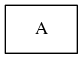
\includegraphics[height=5em]{first_commit.png}
  \caption{First commit}
\end{figure}

\end{frame}

\begin{frame}[fragile]
\frametitle{Tracking changes}

Lets do some stuff.

\vspace{1em}

\begin{lstlisting}[frame=single]
  echo "puts 'Hello Fish'" > hello.rb
  ruby hello.rb
  git commit -m 'Hello Fish?'
  echo 'puts "Hello " + [0x1F431].pack("U*")' > hello.rb
  git commit -am 'Hello?'
  ruby hello.rb
\end{lstlisting}

\begin{figure}[p]
  \centering
  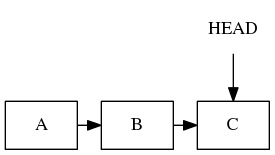
\includegraphics[height=5em]{some_commits.png}
\end{figure}

\end{frame}

\begin{frame}[fragile]
\frametitle{What is HEAD?}

Spoiler: It's the current commit

\vspace{1em}

\begin{lstlisting}[frame=single]
  git branch 'sweet_cat_branch'
  git checkout HEAD~1
  ruby hello.rb
\end{lstlisting}

\begin{figure}[p]
  \centering
  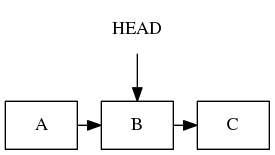
\includegraphics[height=5em]{head.png}
\end{figure}

\end{frame}

\begin{frame}[fragile]
\frametitle{Branching}

\begin{lstlisting}[frame=single]
  git branch "fish_rule"
  git checkout "fish_rule"
  echo 'puts "Fish Rule"' >> hello.rb
  ruby hello.rb
  git commit -am "Fish are way better then cats"
  echo '["Fish live in the ocean."]' >> fish_facts.json
  git add fish_facts.json
  git commit -am "Some fish facts"
  git log
\end{lstlisting}

\begin{figure}[p]
  \centering
  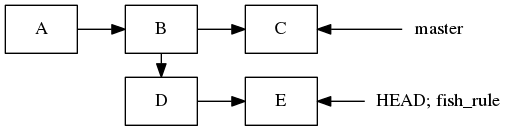
\includegraphics[height=5em]{fish.png}
\end{figure}

\end{frame}


\begin{frame}[fragile]
\frametitle{Merging}

Merging allows you to combine changes

\vspace{1em}

\begin{lstlisting}[frame=single]
  git diff master
  git merge master
\end{lstlisting}

\end{frame}

\begin{frame}[fragile]
\frametitle{Merging}

Merging allows you to combine changes

\vspace{1em}

\begin{lstlisting}[frame=single]
  git diff master
  git merge master
\end{lstlisting}

\vspace{1em}

\begin{lstlisting}[frame=single]
  git status
  cat hello.rb
  git checkout --ours hello.rb 
  git status
  git commit -am "Fish are better"
  git status
\end{lstlisting}

\begin{figure}[p]
  \centering
  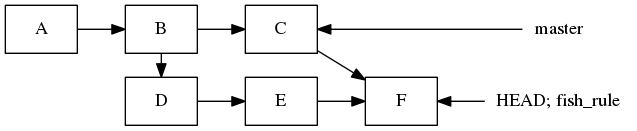
\includegraphics[height=5em]{merge.png}
\end{figure}

\end{frame}

\begin{frame}[fragile]
\frametitle{Fast Forwarding}

Fish are super awesome, they're going into production.

\vspace{1em}

\begin{lstlisting}[frame=single]
 git checkout master
 git merge fish_rule
 git status
 git log
\end{lstlisting}

\begin{figure}[p]
  \centering
  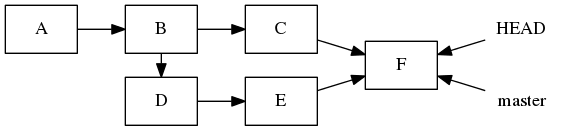
\includegraphics[height=5em]{fast_forward.png}
\end{figure}

\end{frame}

\begin{frame}[fragile]
\frametitle{Push and Pull}

Push moves your current branch onto a remote server

\vspace{1em}

\begin{lstlisting}[frame=single]
  git push 
\end{lstlisting}

\vspace{1em}

Pull gets (merges!) your current branch from the remote server

\vspace{1em}

\begin{lstlisting}[frame=single]
  git pull 
\end{lstlisting}

\end{frame}

\begin{frame}

\frametitle{That's it (basically)}

\begin{figure}[p]
  \centering
  
\includegraphics[height=15em]{howard.jpg}
  \caption{Sure sure, you can use git, but can you really use git?}
\end{figure}

\end{frame}

\begin{frame}[fragile]

\frametitle{git praise (It's really called git blame)}

Credit where credit is due.

\vspace{1em}

\begin{lstlisting}[frame=single]
  git config --global alias.praise blame
  git praise fish_facts.json
\end{lstlisting}

\vspace{1em}

\begin{itemize}
  \item{Who can I ask about this?}
  \item{How old is this code?}
  \item{What was the most recent change?}
\end{itemize}

\end{frame}

\begin{frame}[fragile]

\frametitle{git bisect}

Find out the exact commit that broke something.

\vspace{1em}

\begin{lstlisting}[frame=single]
  git bisect start
  git bisect bad
  git checkout <known good branch>
  git bisect good
\end{lstlisting}

When it works it's magical, try it out.

\end{frame}

\begin{frame}[fragile]

\frametitle{git diff revisited}

Diff is your friend; it is way more powerful then you might know.

\vspace{1em}

\begin{lstlisting}[frame=single]
  git checkout -b "cats_strike_again"
  mv fish_facts.json cat_facts.json
  sed 's/Fish/Cats/g' cat_facts.json
  git checkout sweet_cat_branch -- hello.rb
  ruby hello.rb
  git commit -am "Cat 3.0 is way faster"
  git commit --amend -m "Cat 3.0! fish sucks!"
\end{lstlisting}

\vspace{1em}

\begin{lstlisting}[frame=single]
  git diff master@{10.minutes.ago} cats_strike_again
  git diff master~4 -- hello.rb
  git diff HEAD cats_strike_again
\end{lstlisting}

\end{frame}

\begin{frame}[fragile]

\frametitle{git log revisited}

Git log also has super powers.

\vspace{1em}

\begin{lstlisting}[frame=single]
  git log --author="andrewb" --pretty=full   
  git log -p -S "Fish"
  git log --after={15.minutes.ago}
\end{lstlisting}

\begin{itemize}
  \item{Who's deleting the most code?}
  \item{What was that code I wrote last tuesday?}
  \item{Who added this feature and who uses it?}
\end{itemize}
    
\end{frame}

\begin{frame}[fragile]
\frametitle{git rebase}

\begin{lstlisting}[frame=single]
  git checkout master
  git branch dog
  touch foo
  git add foo
  git commit -m "Added foo"
  git checkout dog
  ls
  touch woof
  git add woof
  git commit -m "Added woof"
\end{lstlisting}

\begin{figure}[p]
  \centering
  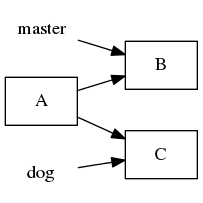
\includegraphics[height=5em]{dog.png}
\end{figure}

\end{frame}

\begin{frame}[fragile]
\frametitle{git rebase}

Subtly different from a merge! Can be used to produce a git history with no merge conflict commits.

\vspace{1em}

\begin{lstlisting}[frame=single]
  git rebase master
\end{lstlisting}

\begin{figure}[p]
  \centering
  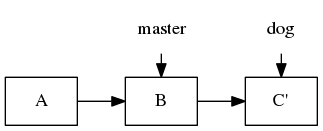
\includegraphics[height=5em]{rebase.png}
\end{figure}

\end{frame}

\begin{frame}[fragile]
\frametitle{git cherrypick}
  
\vspace{1em}

\begin{lstlisting}[frame=single]
  touch good_file
  git commit -am "good commit"
  touch bad_file
  git commit -am "bad commit"
  git checkout master
  git cherry-pick <find the good one>
  ls
\end{lstlisting}

\begin{figure}[p]
  \centering
  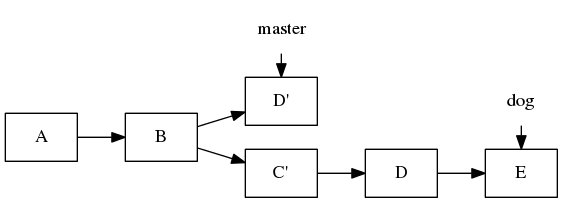
\includegraphics[height=5em]{cherry.png}
\end{figure}

\end{frame}

\begin{frame}[fragile]
\frametitle{Losing your work with delete}

If you never do the likes of this, you're not trying hard enough.

\vspace{1em}

\begin{lstlisting}[frame=single]
  git branch -D dog
  git branch
  git status
  git checkout master
  git status
\end{lstlisting}

\vspace{1em}

\begin{figure}[p]
  \centering
  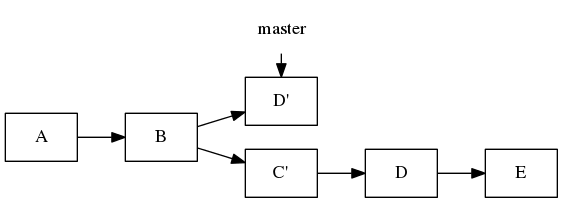
\includegraphics[height=5em]{gone.png}
\end{figure}

\end{frame}

\begin{frame}[fragile]
\frametitle{Reflog to the rescue!}

\vspace{1em}

\begin{lstlisting}[frame=single]
  git reflog
  git checkout <lost commit>
  git branch lost_dog
\end{lstlisting}

\vspace{1em}

\begin{figure}[p]
  \centering
  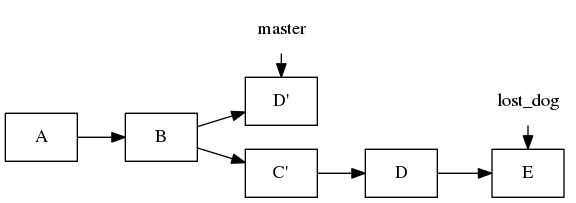
\includegraphics[height=5em]{returned.png}
\end{figure}

\end{frame}

\begin{frame}[fragile]
\frametitle{Losing your work with reset}

\begin{lstlisting}[frame=single]
  touch the_file
  git add the_file
  git reset --hard
  ls
\end{lstlisting}

\vspace{1em}

It's gone. Really gone.

\vspace{1em}

\begin{lstlisting}[frame=single]
  git checkout -- .
\end{lstlisting}

\end{frame}

\begin{frame}[fragile]

\frametitle{So what?}

\begin{itemize}
  \item{Commit frequently and never lose your work again}
  \item{Use descriptive commit messages and never forget what you were doing}
  \item{Merge master often, work on fast moving projects}
  \item{Work from any machine with an internet connection}
  \item{Navigate code smarter and find bugs faster}
  \item{Code metadata, exactly what, when, why, and who}
  \item{Stop time, go work on something else, and pick it right back up again}
\end{itemize}
    
\end{frame}

\end{document}
